% ============================================================
% From Vision to Reality:
% A Formal Theory of Embodied Manifestation
% Daniel Ray Edgar
% ============================================================
\documentclass[11pt]{article}

\usepackage[T1]{fontenc}
\usepackage{lmodern}
\usepackage[margin=1.25in]{geometry}
\usepackage{natbib}
\usepackage{amsmath,amssymb,amsthm}
\usepackage{mathtools}
\usepackage{bm}
\usepackage{xcolor}
\usepackage{hyperref}
\usepackage{booktabs}
\usepackage{array}
\usepackage{tabularx}
\usepackage{longtable}
\usepackage{caption}
\usepackage{microtype}
\usepackage{tikz}
\usetikzlibrary{arrows.meta, positioning, fit, calc, backgrounds}

\definecolor{darkblue}{RGB}{0,60,120}
\definecolor{medblue}{RGB}{0,100,200}
\definecolor{lightblue}{RGB}{220,236,250}
\definecolor{palegreen}{RGB}{225,242,232}
\definecolor{paleyellow}{RGB}{251,242,211}
\definecolor{darkgray}{RGB}{75,75,75}

\hypersetup{
  colorlinks=true,
  linkcolor=darkblue,
  citecolor=darkblue,
  urlcolor=medblue
}

\theoremstyle{plain}
\newtheorem{theorem}{Theorem}[section]

\theoremstyle{definition}
\newtheorem{definition}[theorem]{Definition}
\newtheorem{prediction}{Prediction}

\newcommand{\Aset}{\mathcal{A}}
\newcommand{\Pset}{\Pi}
\newcommand{\doop}{\operatorname{do}}

\title{%
  \vspace{-0.5cm}
  \textbf{From Vision to Reality:}\\[3pt]
  \textbf{A Formal Theory of Embodied Manifestation}
  \vspace{0.3cm}
}

\author{Daniel Ray Edgar}
\date{\normalsize\today}

% ============================================================
\begin{document}
\pagenumbering{gobble}
\maketitle
\thispagestyle{empty}

\begin{abstract}
Every human-made reality exists twice: first as a representation in one or more
minds, then as a physical arrangement produced through action. A building begins as
a plan. A company begins as a model of a future institution. A changed life begins
as an image of a person who does not yet fully exist. This paper develops a concise
theory of that passage from vision to reality.

The central claim is that visualization can change the physical future when it changes
attention, expectation, policy selection, and action. Biological state constrains
which policies a person can reliably execute. Action changes the environment, and
feedback updates both the person and the plan. I formalize this loop with a policy
mixture model and prove three results within it. First, visualization requires a
mediator: if policy and action do not change, an external outcome does not change
under the ordinary causal graph. Second, an embodied state that enables more effective
policies expands the set of reachable futures. Third, repeated well-directed attempts
compound the probability of material success.

The theory integrates evidence from mental imagery, implementation intentions,
placebo physiology, bioelectric signaling, sleep, circadian timing, metabolism,
hydration, inflammation, habits, notifications, and contemplative practice. It also
sets clear boundaries. Quantum effects occur in biology, but this does not establish
voluntary selection of quantum timelines. DNA conducts charge, but this does not make
ordinary language a genetic programming interface. U.S. Patent 6,506,148 and the
Gateway memorandum are genuine primary records of proposed mechanisms and
institutional inquiry, not conclusive experimental validation.

Alchemy, kundalini, theosis, Christ consciousness, and related traditions can be read
as symbolic maps of disciplined transformation. The practical conclusion is strong
without requiring magical causation: imagination supplies direction, the body supplies
capacity, action supplies physical force, and feedback turns a private vision into a
public reality.
\end{abstract}

\newpage
\pagenumbering{arabic}

% ============================================================
\section{The Claim}
% ============================================================

The phrase \emph{manifest your reality} is used for several different claims. One is
ordinary and true: a person imagines a future, organizes behavior around it, and helps
bring it about. Another is possible but underspecified: vivid inner experience may
change health, perception, and performance through mechanisms not yet fully mapped. A
third is much stronger: thought alone selects an external quantum timeline or directly
rearranges matter. These claims should not be treated as one.

This paper defends the first claim, studies the second, and turns the third into a
testable boundary. The resulting view is neither trivial nor magical. Human beings are
not passive observers of a fixed future. They are living causes inside the world.
What they repeatedly represent changes what they notice, prepare for, attempt, build,
and become. Those changes alter later physical states.

The simple causal chain is:

\begin{equation}
\text{vision}
\longrightarrow
\text{embodied state}
\longrightarrow
\text{policy}
\longrightarrow
\text{action}
\longrightarrow
\text{physical change}
\longrightarrow
\text{feedback}.
\label{eq:chain}
\end{equation}

Each arrow matters. Vision without embodiment becomes fantasy. Capacity without
direction becomes unused potential. Intention without policy remains a wish. Policy
without action remains private. Action without feedback becomes repetition without
learning. Manifestation is the complete loop.

This is also why the body matters. A sleep-deprived, inflamed, distracted, or
chronically stressed person does not merely feel worse. That state changes attention,
inhibition, learning, valuation, and the reliability of action. Conversely, recovery,
practice, environmental design, and meaning can enlarge the range of policies that
are available at the decisive moment. Biology is not destiny, but it shapes the menu
from which agency chooses.

% ============================================================
\section{What Manifestation Means}
% ============================================================

The word \emph{reality} needs a precise object. Three levels are sufficient.

\begin{definition}[Mental plane]
The mental plane is the set of internal representations an agent can currently form:
images, concepts, goals, counterfactuals, memories, and models of possible futures.
\end{definition}

\begin{definition}[Embodied plane]
The embodied plane is the agent's present capacity to perceive, regulate, decide,
learn, and act. It includes attention, expectation, emotion, physiological state,
skill, and action readiness.
\end{definition}

\begin{definition}[Physical plane]
The physical plane is the observable world in which actions have consequences:
bodies, objects, documents, money, relationships, institutions, and environments.
\end{definition}

The mental plane is not unreal. A representation is a physical process in a living
nervous system and can be causally important before its object exists. Yet a mental
model is not identical to the world it represents. The imagined house is not a house.
It becomes one only when the representation controls drawings, budgets, contracts,
tools, and coordinated labor.

This distinction gives a professional meaning to \emph{astral visualization}. The
term can describe a vivid symbolic experience in which a desired reality is perceived
as already present. Such experience may carry unusual emotional force or a sense of
self-transcendence \citep{james1902varieties,yaden2017selftranscendent}. The paper
does not require an astral substance. Its causal question is simpler: does the
experience change the embodied policies that later change the world?

\begin{figure}[t]
\centering
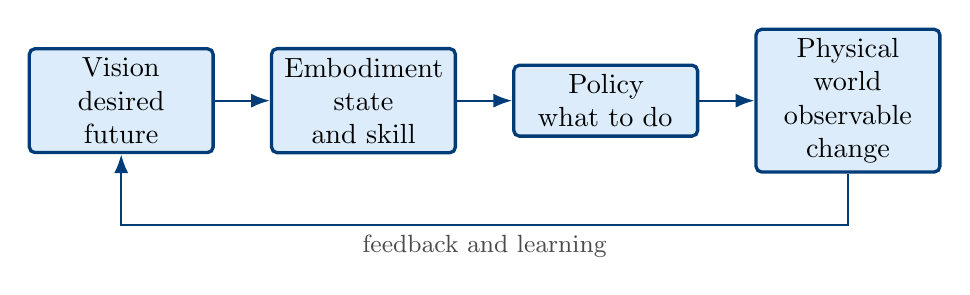
\begin{tikzpicture}[
  node distance=7mm,
  box/.style={
    rounded corners=2pt,
    draw=darkblue,
    very thick,
    minimum height=9mm,
    text width=2.1cm,
    align=center,
    fill=lightblue
  },
  arrow/.style={-{Latex[length=2.4mm]}, thick, darkblue}
]
\node[box] (vision) {Vision\\desired future};
\node[box, right=of vision] (body) {Embodiment\\state and skill};
\node[box, right=of body] (policy) {Policy\\what to do};
\node[box, right=of policy] (world) {Physical world\\observable change};
\draw[arrow] (vision) -- (body);
\draw[arrow] (body) -- (policy);
\draw[arrow] (policy) -- (world);
\draw[arrow] (world.south) -- ++(0,-0.65) -| node[pos=0.25, below, text=darkgray]
  {\small feedback and learning} (vision.south);
\end{tikzpicture}
\caption{The passage from a private representation to a public result. Vision sets
direction; embodiment determines capacity; policy organizes action; physical change
returns evidence.}
\label{fig:loop}
\end{figure}

Manifestation, in the sense defended here, is therefore:

\begin{quote}
\emph{the process by which a represented future changes the policies of an embodied
agent, whose actions increase the probability that the represented future becomes an
observable state of the world.}
\end{quote}

This definition preserves the power of the idea while making it measurable. It also
prevents two errors. The first is fatalism: the future is not fixed because present
action changes its distribution. The second is omnipotence: the agent acts inside
material, social, and probabilistic constraints.

% ============================================================
\section{A Formal Model}
% ============================================================

Let \(V\) denote a visualized target, \(B\) the agent's biological and cognitive
state, \(E\) the environment, \(\pi\) a policy or organized course of action, and
\(Y\) a later physical outcome. The basic identity is:

\begin{equation}
P(Y\mid V,B,E)
=
\sum_{\pi\in\Pset(B,E)}
P\!\left(Y\mid\doop(\pi),B,E\right)
P(\pi\mid V,B,E).
\label{eq:operator}
\end{equation}

The first term inside the sum asks what happens if policy \(\pi\) is executed. The
second asks how likely the agent is to select that policy given the vision, body, and
environment. Visualization has power when it changes the weights assigned to useful
policies. Biology and environment determine which policies are available and whether
they can be executed reliably.

\subsection{The mediation theorem}

\begin{theorem}[Mediation theorem]
Assume the ordinary causal graph
\[
V \longrightarrow \pi \longrightarrow Y,
\]
with \(B\) and \(E\) fixed. If
\[
P(\pi\mid V=v_1,B,E)=P(\pi\mid V=v_2,B,E)
\]
for every policy \(\pi\), then
\[
P(Y\mid V=v_1,B,E)=P(Y\mid V=v_2,B,E).
\]
\end{theorem}

\begin{proof}
Apply Equation~\ref{eq:operator} to \(v_1\) and \(v_2\). The interventional outcome
term \(P(Y\mid\doop(\pi),B,E)\) is the same in both sums because the policy, body, and
environment are fixed. By assumption, the policy weight is also the same for every
\(\pi\). The sums are therefore equal.
\end{proof}

The theorem says something practical and something scientific. Practically, an image
that never changes attention, preparation, choice, or action should not be expected to
change an external result. Scientifically, any reproducible effect on a shielded
external system after every ordinary mediator is fixed would falsify this graph and
require a new causal edge. The theorem does not declare such an edge impossible. It
states what evidence would be needed.

\subsection{The reachable-future theorem}

For reliability threshold \(\rho\), let \(\Pset_\rho(B,E)\) be the set of policies the
agent can execute with at least reliability \(\rho\). For outcome threshold
\(\epsilon\), define the reachable-future set:

\begin{equation}
\Aset_{\epsilon,\rho}(B,E)
=
\left\{
y:
\exists \pi\in\Pset_\rho(B,E)
\text{ with }
P\!\left(y\mid\doop(\pi),B,E\right)\ge\epsilon
\right\}.
\label{eq:reachable}
\end{equation}

\begin{theorem}[Reachable-future theorem]
Let \(B^+\) and \(B^-\) be two embodied states in the same environment. If
\[
\Pset_\rho(B^-,E)\subseteq\Pset_\rho(B^+,E),
\]
and every outcome reachable under \(B^-\) remains at least as likely under the same
policy in \(B^+\), then
\[
\Aset_{\epsilon,\rho}(B^-,E)
\subseteq
\Aset_{\epsilon,\rho}(B^+,E).
\]
If at least one additional policy in \(B^+\) reaches an outcome not reachable in
\(B^-\), the inclusion is strict.
\end{theorem}

\begin{proof}
Take any \(y\in\Aset_{\epsilon,\rho}(B^-,E)\). By definition, some
\(\pi\in\Pset_\rho(B^-,E)\) reaches \(y\) with probability at least \(\epsilon\).
Set inclusion makes the same policy available in \(B^+\), and the probability
assumption preserves the threshold. Thus \(y\in\Aset_{\epsilon,\rho}(B^+,E)\).
If an additional policy reaches a new qualifying outcome, that outcome belongs only
to the second set.
\end{proof}

The result formalizes a familiar experience. When exhaustion removes the policy
\emph{have the difficult conversation calmly}, a relational future disappears from
the reachable set for that moment. When training adds the policy \emph{build and
deploy the prototype}, futures that were once imaginary become reachable. Improved
state does not guarantee an outcome. It changes the set of outcomes for which there
is a credible path.

\subsection{The repetition theorem}

\begin{theorem}[Repetition theorem]
Suppose an agent makes \(n\) conditionally independent attempts at a target, with
success probabilities \(p_1,\ldots,p_n\). The probability of at least one success is
\[
P(\text{success by }n)
=
1-\prod_{t=1}^{n}(1-p_t).
\]
For any attempt with \(0<p_t<1\), adding another attempt with positive probability or
increasing any \(p_t\) strictly increases the cumulative probability.
\end{theorem}

\begin{proof}
The probability that every attempt fails is the product
\(\prod_{t=1}^{n}(1-p_t)\). The complementary event is at least one success. Adding a
factor \(1-p_{n+1}<1\) makes the failure product smaller. Increasing a \(p_t\) also
makes its failure factor smaller. In either case the complement becomes larger.
\end{proof}

Real attempts are not perfectly independent, but the logic survives in richer
models. A clear vision can increase the number of directed attempts, improve their
quality, and make feedback useful. Small changes then accumulate. What looks
retrospectively like a sudden manifestation is often the visible threshold of a long
sequence.

\begin{figure}[t]
\centering
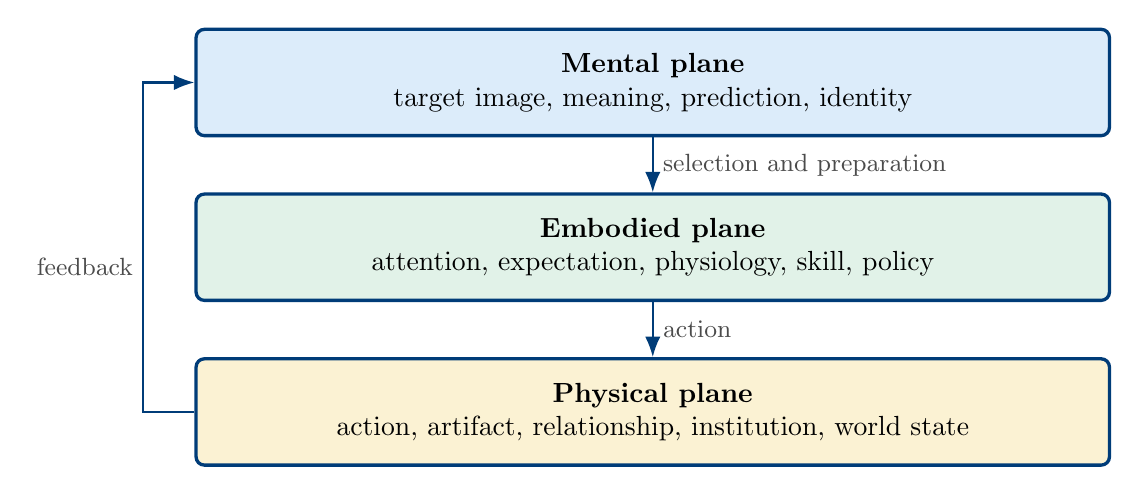
\begin{tikzpicture}[
  plane/.style={
    rounded corners=3pt,
    very thick,
    minimum width=11.6cm,
    minimum height=1.35cm,
    align=center
  },
  arrow/.style={-{Latex[length=2.6mm]}, thick, darkblue}
]
\node[plane, draw=darkblue, fill=lightblue] (mental)
  {\textbf{Mental plane}\\target image, meaning, prediction, identity};
\node[plane, draw=darkblue, fill=palegreen, below=7mm of mental] (embodied)
  {\textbf{Embodied plane}\\attention, expectation, physiology, skill, policy};
\node[plane, draw=darkblue, fill=paleyellow, below=7mm of embodied] (physical)
  {\textbf{Physical plane}\\action, artifact, relationship, institution, world state};
\draw[arrow] (mental) -- node[right, text=darkgray]{\small selection and preparation} (embodied);
\draw[arrow] (embodied) -- node[right, text=darkgray]{\small action} (physical);
\draw[arrow] (physical.west) -- ++(-0.65,0) |- node[pos=0.22, left, text=darkgray]
  {\small feedback} (mental.west);
\end{tikzpicture}
\caption{The three planes are not competing universes. They are stages in one causal
process. A private model becomes physically consequential through an embodied agent.}
\label{fig:planes}
\end{figure}

% ============================================================
\section{How Vision Enters the Body}
% ============================================================

The formal model leaves an empirical question: how can a representation change policy
weights? Four mechanisms are well supported.

\paragraph{Attention.}
A goal changes the relevance map through which the world is sampled. Once a target is
represented clearly, cues related to it become easier to notice, encode, and retrieve.
This is not the universe sending signs. It is selective perception serving an active
model. Because no person can process every available signal, relevance is a genuine
causal resource.

\paragraph{Rehearsal.}
Mental imagery recruits parts of the systems used in perception and action. In one
study, kinesthetic imagery training changed brain signals and increased strength
\citep{yao2013imagery}. The careful inference is not that imagination replaces
practice. It is that simulation can prepare the controller that practice uses.
Effective visualization therefore includes process, obstacles, and response, not only
the pleasure of completion.

\paragraph{Expectation.}
Expectations can alter internal physiology. Placebo research has connected expectation
to dopamine release in Parkinson's disease and to measurable changes in pain-related
brain activity \citep{delafuente2001placebo,wager2004placebo}. These results do not
show that belief can cure any disease. They do show that meaning is not outside
biology. A representation can become a physiological input.

\paragraph{Implementation.}
A goal becomes much more executable when translated into an if-then rule: \emph{if
situation \(X\) occurs, I will perform action \(A\)}. Implementation-intention
research shows why desire alone is weaker than a prepared policy
\citep{sheeran2005implementation}. Visualization supplies direction; implementation
intentions supply grammar.

The same logic applies to identity. Repeatedly imagining oneself as a builder, athlete,
parent, leader, or contemplative can influence which actions feel consistent with the
self-model. That effect can be constructive or delusional. The difference is
feedback. A useful identity produces observable evidence and updates when reality
disagrees.

% ============================================================
\section{The Body Changes What Is Possible}
% ============================================================

The human body is not merely a vehicle carrying an independent mind. It is part of the
decision system. Neurons signal electrically; cells maintain membrane potentials;
tissues coordinate through chemical, mechanical, and bioelectric channels. Work on
development and regeneration shows that bioelectric patterns participate in large-scale
anatomical organization \citep{levin2021bioelectric,durant2019planarian}. This is
strong evidence for biological information processing. It is not, by itself, evidence
that the body receives semantic commands from a cosmic field.

Several ordinary state variables change the reachable policy set.

\paragraph{Sleep and timing.}
Sleep deprivation impairs decisions that require updating from feedback
\citep{whitney2015sleep}. Circadian misalignment impairs performance in
task-dependent ways \citep{chellappa2018circadian}. A person may still hold the same
dream while losing the ability to learn from the day's evidence. Rest is therefore not
separate from manifestation. It protects the update step.

\paragraph{Energy, hydration, and inflammation.}
Metabolic state can alter decisions under risk \citep{symmonds2010metabolic}. Mild
dehydration has been associated with changes in cognition and mood
\citep{ganio2011dehydration,armstrong2012dehydration}. Experimental immune activation
can change neurobehavioral function \citep{grigoleit2011endotoxin}. These findings do
not mean every bad choice is caused by a biomarker. They show why state cannot be
excluded from a theory of agency.

\paragraph{Food and the gut-brain axis.}
In a randomized inpatient trial, ultra-processed diets caused higher calorie intake
and weight gain than minimally processed diets offered under matched conditions
\citep{hall2019ultraprocessed}. Microbiome interventions can affect reported emotional
and neural measures, although results remain intervention-specific
\citep{bagga2018probiotics}. Nutrition influences capacity through ordinary metabolic,
endocrine, immune, and neural pathways. No quantum-field explanation is required.

\paragraph{Attention environments.}
Phone notifications impose measurable attentional costs even when the user does not
respond \citep{stothart2015notifications,upshaw2022notifications}. Habits are strongly
coupled to stable contexts, and context change can disrupt them \citep{wood2005habits}.
Recommendation systems are explicitly optimized to select what a user sees next
\citep{covington2016youtube}. Processed food and digital distraction do not prove a
single conspiracy to suppress divinity. They do reveal incentive systems that profit
when short-term consumption wins against long-term intention.

This is the grounded meaning of \emph{frequency} and \emph{coherence}. Frequency can
refer literally to oscillation only when a rate is measured. In personal practice it
is better used as a metaphor for a stable pattern of attention, emotion, physiology,
and conduct. Coherence is alignment among goal, state, policy, and action. When those
parts conflict, energy is spent without directed change. When they align, the same
person becomes a more reliable cause.

% ============================================================
\section{Evidence and Boundaries}
% ============================================================

The paper uses four evidence levels. \emph{Established} means replicated causal
evidence or mature physical theory. \emph{Supported} means convergent evidence with
meaningful limits. \emph{Plausible} means a testable extension. \emph{Interpretive}
means philosophical, phenomenological, or theological meaning rather than a laboratory
result. Keeping these levels separate makes the synthesis stronger.

\subsection{DNA, fields, and quantum language}

DNA is genetic material, a regulated polymer, and a medium through which charge
transport can occur \citep{crick1970central,virolainen2023geneenvironment,
zwang2018dnacharge}. Calling it either a code \emph{or} an antenna creates a false
choice. It has several physical and informational properties. The specific claim that
ordinary words semantically program DNA has not been established by blinded,
independent, multilaboratory replication. Even literature sympathetic to a DNA
``phantom effect'' notes the replication problem
\citep{gariaev2011wavegenetics,brill2012phantom}.

The heart produces electrical and magnetic signals. Magnetocardiography measures
fields in the picotesla range \citep{roth2024magnetocardiogram}. Measurement does not
create a privileged three-foot boundary or demonstrate that the field broadcasts
intentions into external reality. Similarly, action potentials involve voltage
changes, but quoting one membrane voltage does not make the body a computer with a
single global bit rate. Published estimates depend on what level is counted, and
recent authors have disputed a proposed ten-bit-per-second behavioral figure
\citep{kandel2021principles,zheng2025bits,sauerbrei2025bits}.

Quantum tunneling occurs in enzyme reactions, and quantum coherence has been studied
in photosynthetic systems \citep{cha1989tunneling,panitchayangkoon2010coherence}.
There is active disagreement about which forms of coherence biology actually uses
\citep{duan2017nolongcoherence}. Quantum-consciousness proposals exist
\citep{hameroff2014orch}, while decoherence calculations show the scale problem faced
by simple macroscopic accounts \citep{tegmark2000decoherence}. The many-worlds
interpretation is an interpretation of quantum mechanics, not a demonstrated method
for a person to choose a preferred branch \citep{vaidman2022manyworlds}.

\subsection{What the patent and Gateway record show}

U.S. Patent 6,506,148 B2, \emph{Nervous System Manipulation by Electromagnetic Fields
from Monitors}, describes a proposed method using pulsed monitor fields in the
0.1 to 15 Hz range \citep{loos2003patent}. Its specification relies substantially on
subject-controlled tuning and subjective responses. A patent grant establishes that
claims passed the applicable legal examination. The USPTO utility requirement is not
a blinded clinical-efficacy standard \citep{uspto2026utility}. Separate neuroscience
does show that visual systems can entrain to video displays under defined conditions
\citep{williams2004displays}. That supports a narrower mechanism, not every claim in
the patent.

The 1983 Department of the Army memorandum \emph{Analysis and Assessment of Gateway
Process}, later released under a CIA archive identifier, is a genuine government
analysis of the Monroe Institute's Gateway framework \citep{mcdonnell1983gateway}.
It combines altered-state practice with Bentov, holographic, and quantum language.
Its conclusion recommends further experiments and describes what might follow
\emph{if} the method works. The document is good evidence that the subject received
serious institutional attention. Its own conditional language prevents it from being
treated as a final report of successful validation.

The patent and memorandum are therefore valuable primary records. They show that
claims about fields and altered consciousness entered formal technical channels.
They do not replace controlled replication. The exact documents used here are
archived with the paper so their wording and provenance remain auditable.

\subsection{Compact claim audit}

\begin{table}[p]
\centering
\small
\caption{What the evidence supports and where it stops.}
\label{tab:audit}
\begin{tabularx}{\textwidth}{>{\raggedright\arraybackslash}p{0.23\textwidth}
  >{\raggedright\arraybackslash}p{0.16\textwidth}
  >{\raggedright\arraybackslash}X}
\toprule
\textbf{Claim} & \textbf{Status} & \textbf{Defensible conclusion} \\
\midrule
Cells use bioelectric signals & Established &
Membrane voltage and bioelectric patterning participate in neural, developmental, and
regenerative processes. \\
\addlinespace
Imagery changes performance & Supported &
Imagery can rehearse controllers and influence later performance; it does not replace
physical execution. \\
\addlinespace
If-then plans improve action & Supported &
Implementation intentions convert goals into context-triggered policies. \\
\addlinespace
Words directly program DNA & Unsupported &
DNA responds to physical and biochemical conditions; semantic word effects lack
independent replication. \\
\addlinespace
The heart emits a field & Established &
The field is measurable; a special consciousness radius or intention broadcast is not
established. \\
\addlinespace
Quantum effects occur in cells & Established &
Specific molecular effects exist; quantum timeline selection by intention does not
follow. \\
\addlinespace
The patent proves manipulation & Documentary &
It proves a method was claimed and granted, not that clinical efficacy was replicated. \\
\addlinespace
Gateway proves astral travel & Documentary &
It proves institutional analysis and proposed testing, not conclusive validation. \\
\addlinespace
Kundalini describes real experience & Interpretive &
The tradition and reported experiences are real objects of study; one universal
physiology is not established. \\
\addlinespace
Sacred secretion is monthly anatomy & Unsupported &
Known cerebrospinal-fluid and pineal physiology do not establish the claimed cycle. \\
\bottomrule
\end{tabularx}
\end{table}

% ============================================================
\section{Ancient Maps of Transformation}
% ============================================================

Long before causal graphs, traditions described transformation with symbolic
architectures. They need not be discarded because some modern anatomical claims are
weak. They can be read at the level where they are strongest.

\paragraph{Alchemy.}
Hermetic and alchemical texts join an image of perfected matter with disciplined
operations of separation, purification, and recombination
\citep{copenhaver1992hermetica,jung1968alchemy}. Psychologically, the pattern is clear:
hold a form, expose the present self to a process, and embody the result. The gold is
both a material aim and a symbol of integrated being.

\paragraph{Kundalini.}
Kundalini traditions provide maps of concentrated practice, ascending energy, and
transformed consciousness \citep{buhnemann2011kundalini,white1996alchemicalbody}.
Contemporary reports describe powerful experiences and lasting effects, although the
data are largely phenomenological \citep{woollacott2021kundalini}. The disciplined
claim is that practices can reorganize experience and identity. The stronger claim of
one universal hidden anatomy remains open.

\paragraph{Theosis and Christ consciousness.}
Christian theosis concerns participation in divine life and transformation into
likeness with God \citep{athanasius2011incarnation,papanikolaou2020theosis}. In the
language of this paper, the highest image of the person becomes a regulative model for
attention, conduct, sacrifice, and love. ``Christ consciousness'' is best treated as
a modern interpretive label for this transformed orientation, not a laboratory
measurement.

\paragraph{Sacred secretion.}
Claims of a universal monthly substance descending from the brain to the sacrum and
returning to the head are not established by known cerebrospinal-fluid or pineal
physiology \citep{hladky2014csf,nichols2018pineal}. Mammalian brains can contain
enzymatic machinery related to DMT biosynthesis, but this does not establish the
popular cycle or its theological interpretation \citep{dean2019dmt}. A practice can
remain meaningful without a false anatomical proof.

Across these traditions, one structure repeats:

\begin{equation}
\text{image}
\longrightarrow
\text{discipline}
\longrightarrow
\text{transformed identity}
\longrightarrow
\text{transformed conduct}.
\label{eq:tradition}
\end{equation}

That structure is compatible with the formal model. The spiritual traditions speak
in symbols about the selection and embodiment of a higher policy. Science can study
the mediators without exhausting the meaning.

% ============================================================
\section{A Practical Materialization Protocol}
% ============================================================

The theory becomes useful only when it changes practice. The following protocol is a
direct translation of the causal model.

\paragraph{1. Specify the physical target.}
State what will be observable if the vision becomes real. ``Become successful'' is
not yet a target. ``Publish the manuscript, place it in the portfolio, and obtain
three qualified reviews'' is. A physical criterion prevents feeling from being
mistaken for completion.

\paragraph{2. Visualize the process and the identity.}
Represent the finished state vividly, then rehearse the process that creates it.
Include the difficult email, the training session, the rejection, the recovery, and
the next attempt. Imagine the kind of person who performs those actions reliably.
Outcome imagery gives direction; process imagery prepares policy.

\paragraph{3. Convert vision into implementation intentions.}
Write if-then rules for the moments that matter: \emph{if it is 7:00 a.m., I open the
manuscript before messages}; \emph{if I receive a rejection, I record the reason and
send the next submission within twenty-four hours}. The rule moves choice from a
future depleted state into a present reflective state.

\paragraph{4. Prepare the body.}
Protect sleep, circadian regularity, hydration, adequate nutrition, movement, and
recovery. Seek clinical care when symptoms require it. This is not wellness decoration.
It is maintenance of the system that must execute the policy.

\paragraph{5. Design the environment.}
Remove cues that trigger the competing identity. Disable unnecessary notifications,
place tools where action begins, reduce friction for desired behavior, and add social
commitments where they help. Willpower is one variable; environment changes the policy
distribution before willpower is tested.

\paragraph{6. Act and produce evidence.}
Create a physical trace each cycle: a page, call, prototype, application, workout,
conversation, or transfer of resources. Evidence tells the nervous system that the
identity is no longer imaginary. It also exposes the plan to the world, where
correction becomes possible.

\paragraph{7. Measure, learn, and repeat.}
Compare the result with the target. Keep the vision stable enough to guide action and
flexible enough to learn. Update the policy, not merely the affirmation. Repetition
then improves both the quality and number of attempts, which is the mechanism in the
repetition theorem.

Contemplative practice can support several steps. Meditation has been associated with
differences in default-mode activity, self-regulation, and, in some contexts,
transcriptional measures \citep{brewer2011meditation,vago2012sart,black2013meditation}.
The responsible conclusion is not that meditation guarantees external outcomes. It
can reduce automaticity, stabilize attention, and change the agent who meets the next
choice.

The protocol is intentionally ordinary in its mechanics and extraordinary in its
implication. A reality that does not yet exist can organize present matter through a
living person. The future reaches backward as information in a model; the person
carries that information forward as action.

% ============================================================
\section{Predictions and Conclusion}
% ============================================================

A theory earns credibility by risking failure. The following predictions separate the
model from unfalsifiable affirmation.

\begin{prediction}
Process visualization combined with implementation intentions will outperform
outcome visualization alone on externally scored goals. The advantage will be
mediated by action frequency and execution quality.
\end{prediction}

\begin{prediction}
Restoring sleep and circadian regularity in disrupted participants will expand
measured policy generation, feedback updating, and execution reliability on defined
tasks.
\end{prediction}

\begin{prediction}
Notification removal and context redesign will improve intentional control most in
participants whose baseline behavior is strongly cue-driven.
\end{prediction}

\begin{prediction}
Repeated directed attempts will explain apparent ``sudden'' manifestations better
than outcome imagery alone when the action history is measured prospectively.
\end{prediction}

\begin{prediction}
Semantic DNA programming will fail blinded, multilaboratory testing unless a
meaning-specific effect survives energy matching, translation, sham exposure, and
open raw-data review.
\end{prediction}

\begin{prediction}
Longitudinal measurement will not reveal one universal monthly
brain-to-sacrum-to-brain secretion cycle across healthy adults.
\end{prediction}

\begin{prediction}
Contemplative practice will change selected measures of attention, regulation, and
self-transcendence through measurable mediators, but it will not reliably alter
shielded random physical outcomes.
\end{prediction}

The final claim can now be stated simply. Human beings are powerful, but their power
is not well described as omnipotent thought. It is the power to model what is absent,
reorganize themselves around that model, and apply directed force to the world. The
mind supplies a future before the future is physical. The body determines whether the
future can be carried. Action gives the image public consequence. Feedback corrects
the difference between desire and reality.

This is how the mental plane descends into the physical plane. Not by skipping
causality, but by entering it. Not every dream will materialize, because other agents,
chance, time, and material constraints are real. Yet no designed future arrives
without first being represented. The image is not the finished world. It is the first
causal form of that world.

\bibliographystyle{plainnat}
\bibliography{refs}

\end{document}
